%%%%%%%%%%%%%%%%%%%%%%%%%%% asme2e.tex %%%%%%%%%%%%%%%%%%%%%%%%%%%%%%%
% ASME-format project report
%%%%%%%%%%%%%%%%%%%%%%%%%%%%%%%%%%%%%%%%%%%%%%%%%%%%%%%%%%%%%%%%%%%%%%

\documentclass[twocolumn,10pt]{asme2e}
\special{papersize=8.5in,11in}

\usepackage{graphicx}
\usepackage{url}
\usepackage{placeins}
\usepackage{balance}

\setlength{\textfloatsep}{8pt plus 2pt minus 2pt}
\setlength{\dbltextfloatsep}{8pt plus 2pt minus 2pt}
\setlength{\floatsep}{6pt plus 2pt minus 2pt}

\confshortname{ID5130}
\conffullname{High Performance Computing Course Project}
\confdate{5}
\confmonth{May}
\confyear{2026}
\confcity{Chennai}
\confcountry{India}
\papernum{ID5130-PARALLEL-OS-UTILS}

\title{A DISTRIBUTED AND PARALLEL IMPLEMENTATION OF CORE OS UTILITIES USING OPENMP AND OPENMPI}

\author{Paurush Kumar
    \affiliation{
    Roll No. NA22B002\\
    Indian Institute of Technology Madras\\
    Chennai, Tamil Nadu, India
    }
}

\author{Akshay Pratap Singh
    \affiliation{
    Roll No. CE21B006\\
    Indian Institute of Technology Madras\\
    Chennai, Tamil Nadu, India
    }
}

\begin{document}

\maketitle

%%%%%%%%%%%%%%%%%%%%%%%%%%%%%%%%%%%%%%%%%%%%%%%%%%%%%%%%%%%%%%%%%%%%%%
\begin{abstract}
{\it This work presents \texttt{pfind} and \texttt{pgrep}, parallel C++ replacements for common file-system search utilities. The tools are implemented in three modes: a project serial baseline, an OpenMP-only version, and a hybrid OpenMPI+OpenMP version. POSIX directory traversal is used for low-overhead path discovery, OpenMP parallelizes seed-subtree traversal and file scanning, and MPI distributes seed work across ranks. For content search, \texttt{pgrep} uses buffered fixed-string matching for small files and streaming Boyer-Moore search for files larger than 1 MiB. Two synthetic workloads were evaluated: a deep many-small-file tree and a large-content tree. Results show clear speedup against the project serial baseline, OpenMP wall-clock speedups over GNU \texttt{find}/\texttt{grep} in several configurations, and hybrid MPI+OpenMP internal-time scaling, with wall-clock MPI performance limited by launch overhead.}
\end{abstract}

%%%%%%%%%%%%%%%%%%%%%%%%%%%%%%%%%%%%%%%%%%%%%%%%%%%%%%%%%%%%%%%%%%%%%%
\begin{nomenclature}
\entry{$T_1$}{Runtime of the project serial implementation}
\entry{$T_p$}{Runtime with $p$ parallel workers or a rank-thread configuration}
\entry{$S_p$}{Speedup, $S_p=T_1/T_p$}
\entry{$E_p$}{Parallel efficiency, $E_p=S_p/p$}
\entry{$B$}{Bytes read by \texttt{pgrep}}
\entry{$R$}{MPI rank count}
\entry{$N_t$}{OpenMP thread count per rank}
\entry{MPI}{Message Passing Interface}
\entry{OpenMP}{Shared-memory directive and runtime API}
\entry{POSIX}{Portable Operating System Interface}
\end{nomenclature}

%%%%%%%%%%%%%%%%%%%%%%%%%%%%%%%%%%%%%%%%%%%%%%%%%%%%%%%%%%%%%%%%%%%%%%
\section*{INTRODUCTION}

The Unix utilities \texttt{find} and \texttt{grep} are standard tools for locating files and searching file contents. They are highly optimized production utilities, but their normal command-line use is still fundamentally a single-process execution model. Modern systems, however, commonly provide many CPU cores, and cluster environments provide multiple nodes. The goal of this project was to explore whether high-performance computing techniques can be applied to this operating-system style workload.

This report describes two tools. The first, \texttt{pfind}, searches file and directory names in a recursive directory tree. In the experiments it is compared with GNU \texttt{find -name}. The second, \texttt{pgrep}, searches file contents recursively and reports the names of matching files. It is compared with GNU \texttt{grep -RIl}. The final implementation differs from the original project abstract in two important ways. First, the final evaluation was performed locally with MPI ranks on the same machine rather than on a two-node Ethernet cluster. Second, \texttt{pgrep} no longer loads all large files into memory; large files are searched by streaming chunks with overlap.

The main contributions are: (i) separate serial, OpenMP, and MPI+OpenMP binaries for fair comparison; (ii) POSIX-based traversal using \texttt{opendir}, \texttt{readdir}, and \texttt{lstat}; (iii) OpenMP parallel traversal and file-level content search; (iv) MPI seed-work distribution; (v) streaming Boyer-Moore search for large-file fixed-string matching; and (vi) repeatable benchmarking with wall-clock time, internal tool time, match counts, and throughput.

%%%%%%%%%%%%%%%%%%%%%%%%%%%%%%%%%%%%%%%%%%%%%%%%%%%%%%%%%%%%%%%%%%%%%%
\section*{BACKGROUND}

GNU \texttt{find} searches a directory hierarchy and evaluates expressions such as name tests on each discovered path \cite{gnu_find}. GNU \texttt{grep} searches input for lines or files containing a pattern; in this work the reference command is \texttt{grep -RIl}, which recursively searches files and prints only file names containing a match \cite{gnu_grep}.

OpenMP provides a shared-memory programming model for C/C++ and Fortran, allowing loop iterations or tasks to be distributed across threads on one node \cite{openmp_spec}. MPI provides a distributed-memory programming model in which independent processes communicate explicitly \cite{mpi_standard}. These models are complementary: MPI can distribute independent subtrees across ranks, while OpenMP can exploit cores within each rank.

For fixed-string content search, large files use the C++17 \texttt{std::boyer\_moore\_searcher}, which implements the Boyer-Moore string searching algorithm \cite{cpp_bm}. Boyer and Moore's original algorithm preprocesses the pattern and often skips ahead by multiple characters during mismatches, reducing the average number of examined text characters for practical search workloads \cite{boyer_moore}. In this project the algorithm is not reimplemented manually; it is used through the C++ standard library searcher interface.

%%%%%%%%%%%%%%%%%%%%%%%%%%%%%%%%%%%%%%%%%%%%%%%%%%%%%%%%%%%%%%%%%%%%%%
\section*{PROBLEM STATEMENT AND OBJECTIVES}

The problem is to accelerate recursive file-system queries while preserving the basic output semantics used for benchmarking. For \texttt{pfind}, the query is a substring match on the base name of each file or directory. For \texttt{pgrep}, the query is a fixed text pattern in file contents, with optional regex support retained as a slower path.

The objectives are:

\begin{enumerate}
\item Build working serial, OpenMP-only, and MPI+OpenMP versions of both tools.
\item Compare parallel performance against the project serial baseline.
\item Use GNU \texttt{find} and GNU \texttt{grep} as external reference baselines.
\item Report both end-to-end wall-clock time and internal traversal/search time.
\item Evaluate two different workload types: deep traversal and large-content search.
\item Validate correctness by comparing match counts and outputs against GNU utilities.
\end{enumerate}

%%%%%%%%%%%%%%%%%%%%%%%%%%%%%%%%%%%%%%%%%%%%%%%%%%%%%%%%%%%%%%%%%%%%%%
\section*{IMPLEMENTATION}

\subsection*{Program Variants}

The build produces six executables. \texttt{pfind\_serial} and \texttt{pgrep\_serial} are compiled without OpenMP and MPI and serve as the primary speedup baselines. \texttt{pfind\_omp} and \texttt{pgrep\_omp} use OpenMP but are launched directly, without \texttt{mpirun}. \texttt{pfind} and \texttt{pgrep} are the hybrid MPI+OpenMP binaries and are launched with \texttt{mpirun -np R}. Therefore, in the plots, labels of the form $1\times N_t$ for OpenMP binaries denote one process and $N_t$ threads, not an MPI launch.

\subsection*{Traversal}

Both tools first decompose the input roots into seed work. The traversal hot path uses POSIX interfaces. Metadata is obtained by \texttt{lstat}; directories are opened with \texttt{opendir}; children are enumerated by \texttt{readdir} \cite{posix_readdir}. This avoids the overhead and reduced control of \texttt{std::filesystem::directory\_iterator} in the inner traversal loop. \texttt{std::filesystem::path} is still used as a path container, but not for directory iteration.

The local traversal supports breadth-first or depth-first behavior using a deque of pending paths. OpenMP parallelizes traversal over seed work items using dynamic scheduling. Each thread accumulates local matches and metrics, then merges them into rank-local totals.

\subsection*{MPI Work Distribution}

Rank 0 expands the top of the tree into seed work items. These seed paths are distributed round-robin across MPI ranks. Each rank then traverses only its assigned seed paths using OpenMP. After local work completes, matching path strings and metrics are gathered back to rank 0. Metrics are reduced using sums for counts and bytes, and the maximum rank time for internal elapsed time.

\subsection*{Content Search}

\texttt{pgrep} separates file discovery from content search. First, traversal returns candidate regular files. Second, those files are searched in parallel with OpenMP. For files up to 1 MiB, the implementation reads the file into a string and uses the standard fixed-string search path. For files larger than 1 MiB, the implementation reads 1 MiB chunks, keeps an overlap of $m-1$ bytes where $m$ is the pattern length, and applies Boyer-Moore search to each chunk window. The overlap is necessary because a match may begin near the end of one chunk and finish in the next chunk.

Regex mode is supported by \texttt{--regex}, but benchmark runs use fixed-string mode. Regex is deliberately isolated behind a branch so it does not affect the fixed-string benchmark path.

%%%%%%%%%%%%%%%%%%%%%%%%%%%%%%%%%%%%%%%%%%%%%%%%%%%%%%%%%%%%%%%%%%%%%%
\section*{ALGORITHMS}

Figure~\ref{fig_algorithm} summarizes the hybrid algorithm.

\begin{figure}[t]
\begin{center}
\fbox{\begin{minipage}{3.1in}
\small
\textbf{Hybrid pfind/pgrep workflow}\\
1. Rank 0 receives input roots.\\
2. Rank 0 expands roots into seed work items.\\
3. Seed items are distributed round-robin to ranks.\\
4. Each rank starts $N_t$ OpenMP threads.\\
5. Threads traverse assigned seed paths using BFS/DFS.\\
6. For \texttt{pfind}, filename predicates are applied during traversal.\\
7. For \texttt{pgrep}, files are collected and then searched in parallel.\\
8. Matching paths are gathered to rank 0.\\
9. Metrics are reduced and one CSV row is written.
\end{minipage}}
\end{center}
\caption{PSEUDOCODE SUMMARY OF THE HYBRID MPI+OPENMP SEARCH WORKFLOW.}
\label{fig_algorithm}
\end{figure}

The project reports speedup and efficiency as follows. Speedup is
\begin{equation}
S_p = \frac{T_1}{T_p},
\label{eq_speedup}
\end{equation}
Parallel efficiency is
\begin{equation}
E_p = \frac{S_p}{p}.
\label{eq_efficiency}
\end{equation}
For OpenMP-only runs, $p=N_t$. For hybrid runs, a natural worker count is $p=R N_t$, although the plots report configurations as $R \times N_t$ because MPI startup overhead and rank-level work distribution make pure worker-count efficiency less direct. For context, Amdahl's fixed-size model is
\begin{equation}
S_A(p)=\frac{1}{f+(1-f)/p},
\label{eq_amdahl}
\end{equation}
where $f$ is the serial fraction. Gustafson-Barsis scaled speedup is
\begin{equation}
S_G(p)=p-\alpha(p-1),
\label{eq_gustafson}
\end{equation}
where $\alpha$ is the serial fraction in the scaled workload. Since the experiments in this report keep each dataset fixed and vary ranks/threads, the results are primarily strong-scaling measurements and are most directly interpreted with Eqn.~(\ref{eq_speedup}) and Eqn.~(\ref{eq_efficiency}). The Karp-Flatt serial fraction,
\begin{equation}
e=\frac{1/S_p-1/p}{1-1/p},
\label{eq_karpflatt}
\end{equation}
is useful for diagnosing overhead, synchronization, and nonideal scaling when $S_p$ is below $p$.

The \texttt{pgrep} throughput is
\begin{equation}
Q = \frac{B}{T},
\label{eq_throughput}
\end{equation}
where $B$ is bytes read and $T$ is either wall-clock or internal elapsed time.

Table~\ref{tab_metric_calc} gives the calculated strong-scaling metrics for representative final runs. The speedups use internal elapsed time so that the measured value reflects traversal and search work rather than MPI process-launch time. The throughput values use Eqn.~(\ref{eq_throughput}) and are shown only for \texttt{pgrep}, since \texttt{pfind} does not read file contents.

\begin{table}[t]
\caption{CALCULATED PARALLEL METRICS FOR REPRESENTATIVE RUNS.}
\begin{center}
\label{tab_metric_calc}
\scriptsize
\begin{tabular}{l c c c c}
\hline
Run & $p$ & $T_p$ & $S_p$ & $E_p$ \\
\hline
Deep \texttt{pfind\_omp} $1\times8$ & 8 & 0.0546 & 4.74 & 0.59 \\
Deep \texttt{pfind} $2\times4$ & 8 & 0.0805 & 3.21 & 0.40 \\
Deep \texttt{pgrep\_omp} $1\times8$ & 8 & 0.2434 & 3.48 & 0.44 \\
Deep \texttt{pgrep} $2\times4$ & 8 & 0.3058 & 2.77 & 0.35 \\
Large \texttt{pgrep\_omp} $1\times8$ & 8 & 0.2298 & 8.13 & 1.02 \\
Large \texttt{pgrep} $2\times4$ & 8 & 0.4470 & 4.18 & 0.52 \\
\hline
\end{tabular}
\end{center}
\end{table}

\begin{table}[t]
\caption{CALCULATED \texttt{pgrep} INTERNAL THROUGHPUT.}
\begin{center}
\label{tab_throughput_calc}
\scriptsize
\begin{tabular}{l c c}
\hline
Dataset and run & $T$ (s) & $Q$ (GB/s) \\
\hline
Deep serial & 0.8479 & 0.84 \\
Deep OpenMP $1\times8$ & 0.2434 & 2.94 \\
Deep MPI+OpenMP $2\times4$ & 0.3058 & 2.34 \\
Large serial & 1.8682 & 2.00 \\
Large OpenMP $1\times8$ & 0.2298 & 16.25 \\
Large MPI+OpenMP $2\times4$ & 0.4470 & 8.35 \\
\hline
\end{tabular}
\end{center}
\end{table}

%%%%%%%%%%%%%%%%%%%%%%%%%%%%%%%%%%%%%%%%%%%%%%%%%%%%%%%%%%%%%%%%%%%%%%
\section*{EXPERIMENTAL METHODOLOGY}

\subsection*{Datasets}

Two synthetic datasets were used. The first, \texttt{deep\_synthetic}, is traversal-heavy: depth 7, fanout 4, four files per directory, and approximately 8 KiB per file. It contains 21,845 directories and 87,380 files. This dataset stresses recursive traversal and many-small-file overhead.

The second, \texttt{large\_content}, is content-search-heavy: depth 5, fanout 3, four files per directory, and file sizes randomly selected from 1,025 KiB to 4,096 KiB. It contains 364 directories and 1,456 files, totaling approximately 3.6 GiB. Since every file is larger than 1 MiB, this dataset exercises the streaming Boyer-Moore path in \texttt{pgrep}.

\subsection*{Benchmark Modes}

Each dataset was benchmarked with GNU reference utilities, project serial binaries, OpenMP binaries, and MPI+OpenMP binaries. Thread counts were $N_t=\{1,2,4,8\}$ and MPI ranks were $R=\{1,2\}$ for the hybrid binary. Each configuration was repeated three times. A warmup run was performed before timing to avoid cold-cache distortion in GNU reference baselines.

The benchmark CSV records wall-clock elapsed time around the whole command, internal elapsed time reported by the tool, directories visited, files visited, bytes read, matches, and errors. Correctness was checked by comparing all variants against GNU \texttt{find} and \texttt{grep}; all final runs had matching counts and zero errors.

%%%%%%%%%%%%%%%%%%%%%%%%%%%%%%%%%%%%%%%%%%%%%%%%%%%%%%%%%%%%%%%%%%%%%%
\section*{RESULTS}

\subsection*{Deep Traversal Dataset}

The deep traversal workload contains many directories and small files. Table~\ref{tab_deep_summary} reports selected results. GNU \texttt{find} averaged 0.1349 s, while GNU \texttt{grep} averaged 0.4969 s after warmup. The OpenMP-only implementations beat GNU wall-clock time at higher thread counts: \texttt{pfind\_omp} at 8 threads reached 0.0602 s, and \texttt{pgrep\_omp} at 8 threads reached 0.2589 s.

\begin{table}[t]
\caption{SELECTED RESULTS ON THE DEEP SYNTHETIC DATASET.}
\begin{center}
\label{tab_deep_summary}
\begin{tabular}{l c c c}
\hline
Config. & Wall & Int. & $S_p$ \\
\hline
\texttt{pfind\_serial} & 0.2626 & 0.2586 & 1.00 \\
\texttt{pfind\_omp} $1\times8$ & 0.0602 & 0.0546 & 4.74 \\
\texttt{pfind} $2\times4$ & 0.3845 & 0.0805 & 3.21 \\
\texttt{pgrep\_serial} & 0.8586 & 0.8479 & 1.00 \\
\texttt{pgrep\_omp} $1\times8$ & 0.2589 & 0.2434 & 3.48 \\
\texttt{pgrep} $2\times4$ & 0.6147 & 0.3058 & 2.77 \\
\hline
\end{tabular}
\end{center}
\end{table}

Figure~\ref{fig_deep_wall} shows wall-clock runtime by configuration. The pure OpenMP curves fall below the GNU baselines for the best \texttt{pfind} and \texttt{pgrep} configurations. The hybrid MPI+OpenMP wall-clock curves improve with more work but remain affected by \texttt{mpirun} launch overhead.

\begin{figure}[t]
\begin{center}
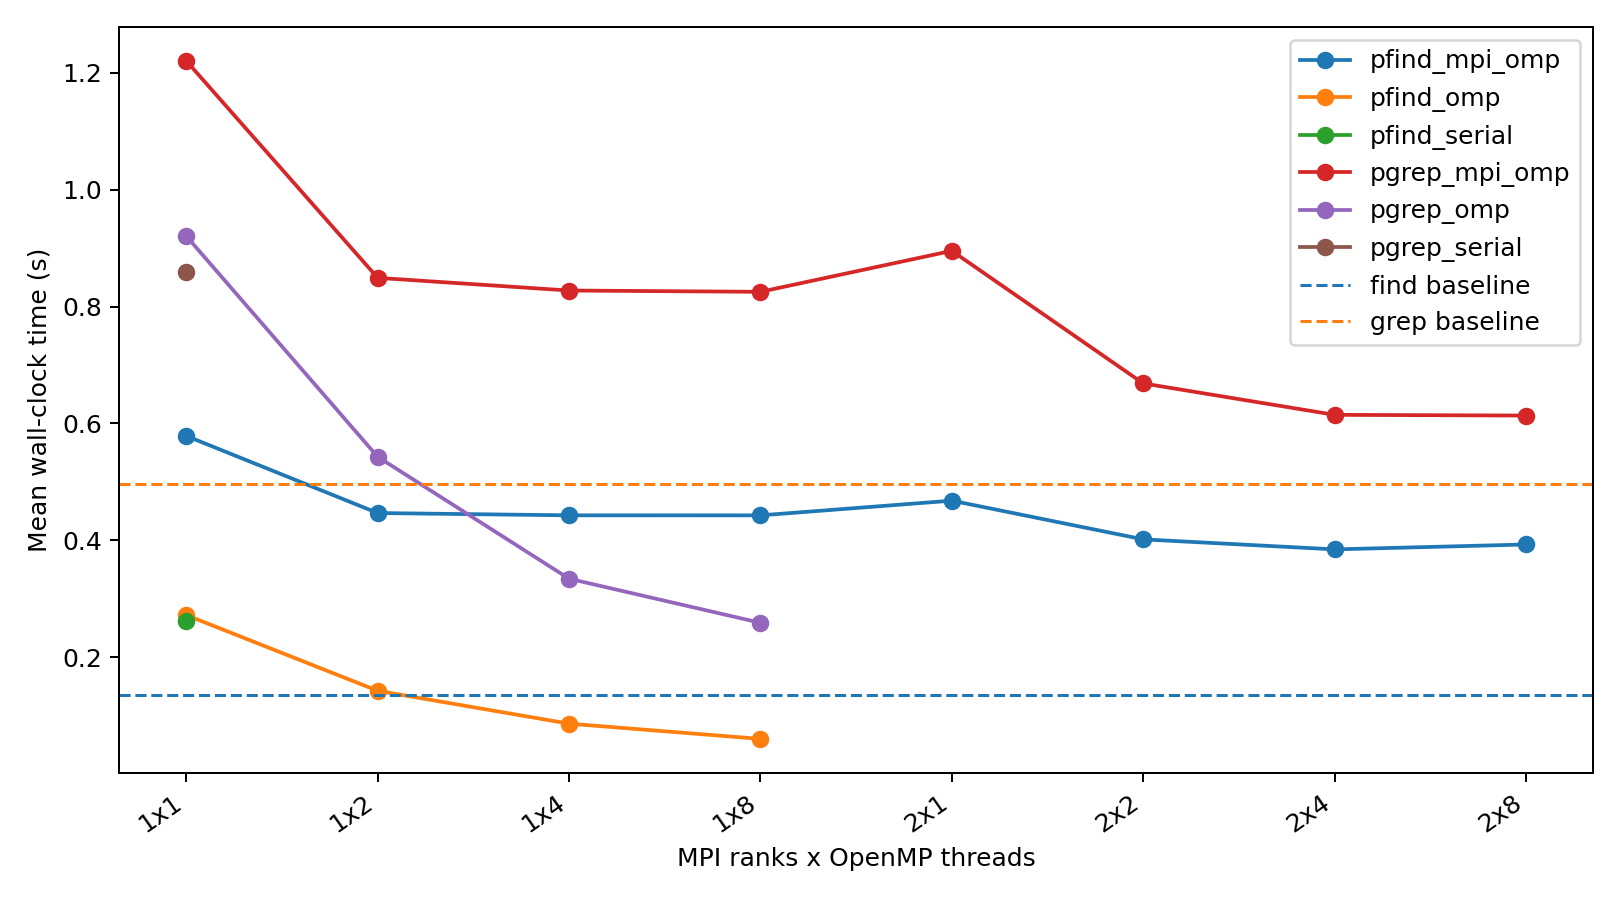
\includegraphics[width=\columnwidth]{../plots/deep_synthetic_final_wallclock/runtime_by_configuration.png}
\end{center}
\caption{WALL-CLOCK RUNTIME ON THE DEEP SYNTHETIC DATASET.}
\label{fig_deep_wall}
\end{figure}

Internal timing removes process-launch effects. In that view, the hybrid implementation shows clearer scaling. For example, \texttt{pgrep} at $2\times4$ reaches 0.3058 s internal time, faster than GNU \texttt{grep}'s 0.4969 s reference time. The internal-time plot is generated in the final plot directory, while Table~\ref{tab_metric_calc} reports the calculated speedup values used for analysis.

\FloatBarrier

\subsection*{Large Content Dataset}

The large-content dataset stresses content scanning rather than directory traversal. GNU \texttt{grep} averaged 1.0936 s. The OpenMP \texttt{pgrep} implementation achieved substantial gains: 0.3948 s at 4 threads and 0.2323 s at 8 threads. The best internal speedup against \texttt{pgrep\_serial} was 8.13 at 8 OpenMP threads. Hybrid \texttt{pgrep} also beat GNU wall-clock time for several configurations, including $2\times4$ with 0.7466 s.

\begin{table}[t]
\caption{SELECTED RESULTS ON THE LARGE-CONTENT DATASET.}
\begin{center}
\label{tab_large_summary}
\begin{tabular}{l c c c}
\hline
Config. & Wall & Int. & $S_p$ \\
\hline
\texttt{pgrep\_serial} & 1.8697 & 1.8682 & 1.00 \\
\texttt{pgrep\_omp} $1\times2$ & 0.7708 & 0.7689 & 2.43 \\
\texttt{pgrep\_omp} $1\times4$ & 0.3948 & 0.3929 & 4.76 \\
\texttt{pgrep\_omp} $1\times8$ & 0.2323 & 0.2298 & 8.13 \\
\texttt{pgrep} $2\times4$ & 0.7466 & 0.4470 & 4.18 \\
\hline
\end{tabular}
\end{center}
\end{table}

Figure~\ref{fig_large_wall} shows wall-clock runtime on the large-content workload. Unlike the deep dataset, \texttt{pgrep} has enough per-file work for the parallel search implementation to overcome overhead more clearly.

\begin{figure}[t]
\begin{center}
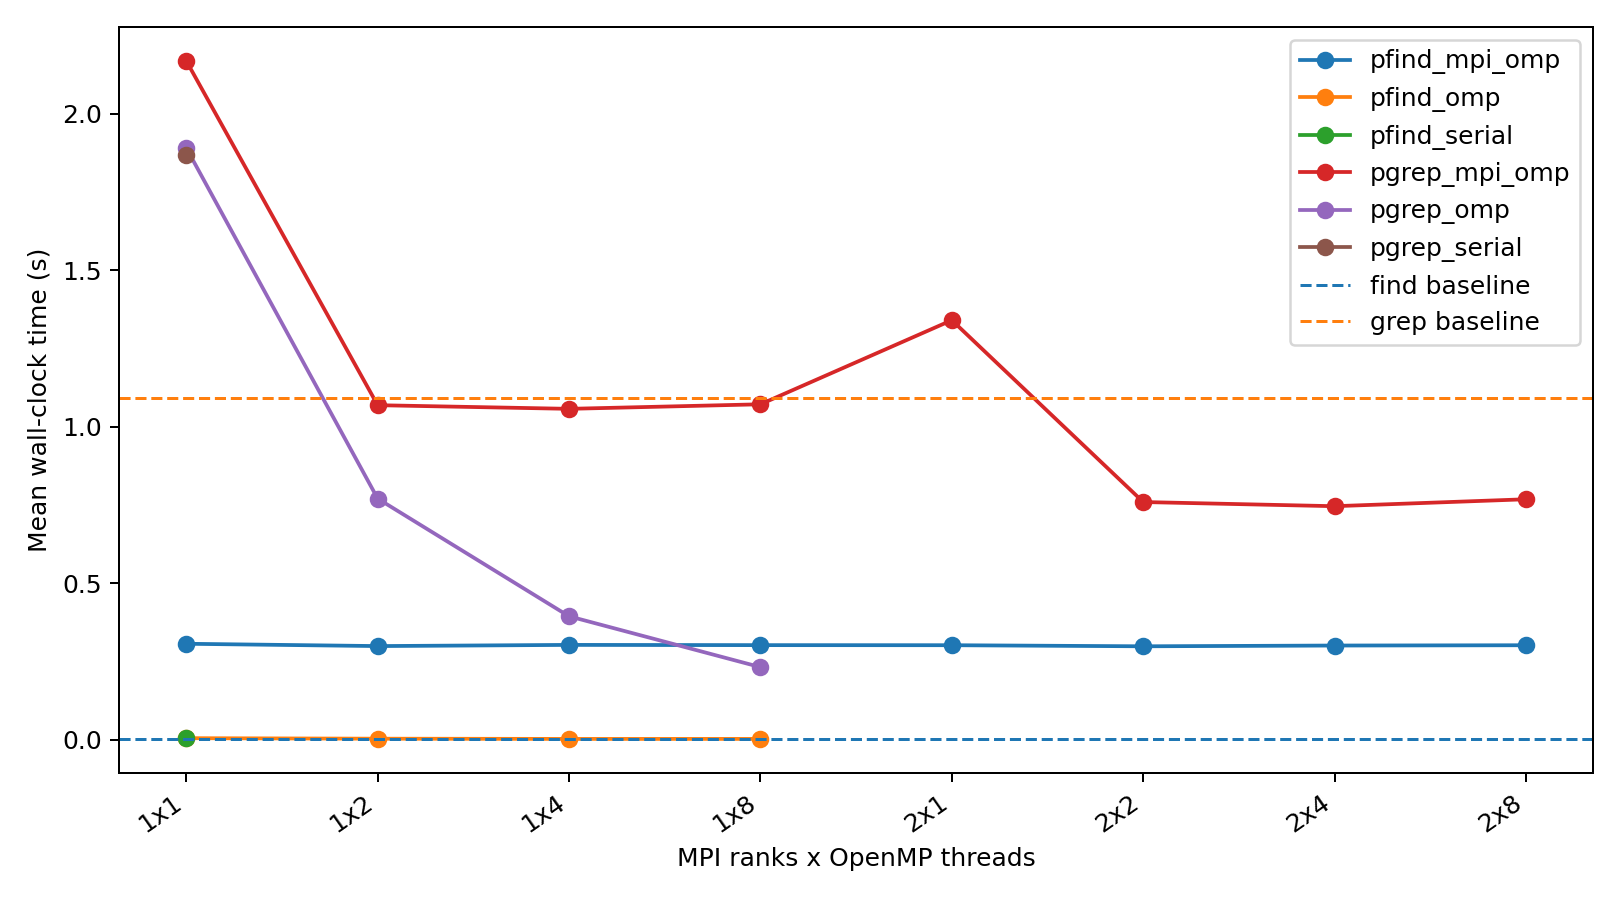
\includegraphics[width=\columnwidth]{../plots/large_content_final_wallclock/runtime_by_configuration.png}
\end{center}
\caption{WALL-CLOCK RUNTIME ON THE LARGE-CONTENT DATASET.}
\label{fig_large_wall}
\end{figure}

Figure~\ref{fig_large_throughput} reports \texttt{pgrep} throughput. The best internal throughput was approximately 16.2 GB/s for \texttt{pgrep\_omp} at 8 threads, compared with about 2.0 GB/s for the project serial implementation. This result demonstrates the benefit of file-level parallel scanning and the large-file fixed-string path.

\begin{figure}[t]
\begin{center}
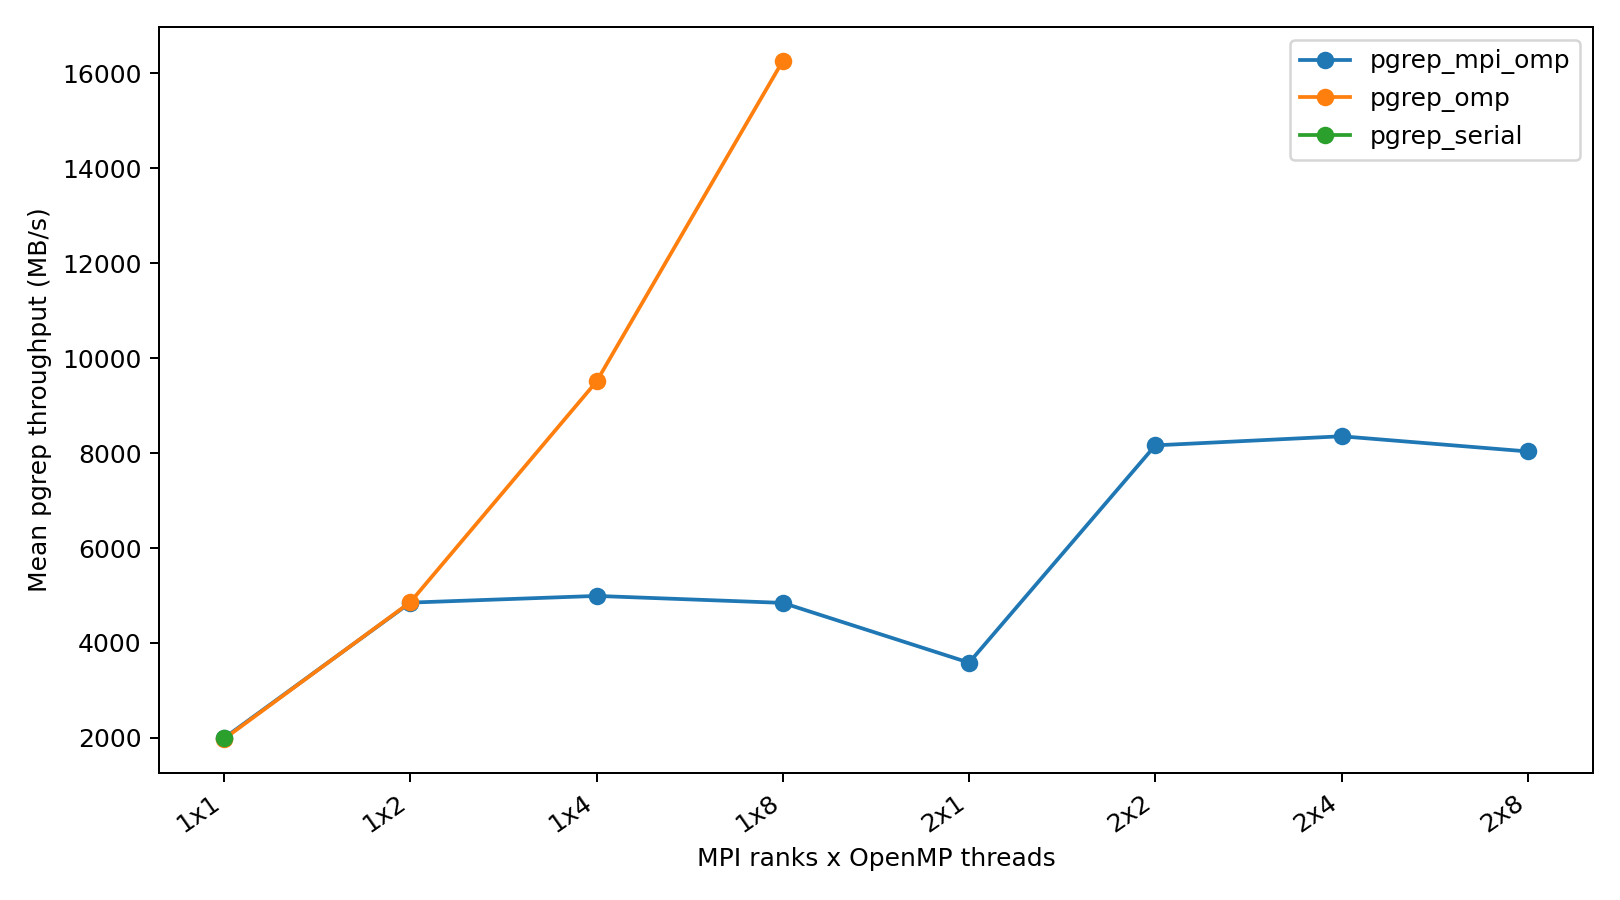
\includegraphics[width=\columnwidth]{../plots/large_content_final_internal/pgrep_throughput.png}
\end{center}
\caption{INTERNAL \texttt{pgrep} THROUGHPUT ON THE LARGE-CONTENT DATASET.}
\label{fig_large_throughput}
\end{figure}

\FloatBarrier

%%%%%%%%%%%%%%%%%%%%%%%%%%%%%%%%%%%%%%%%%%%%%%%%%%%%%%%%%%%%%%%%%%%%%%
\section*{DISCUSSION}

The results show that the best parallel strategy depends on workload structure. The deep dataset has many small files and many directories. In this case, traversal and file-open overhead dominate, and OpenMP gives a strong benefit by processing independent seed paths and files concurrently. MPI internal time also improves, but end-to-end wall-clock time remains limited by launch overhead for single-query runs. For example, \texttt{pfind\_omp} at 8 threads gives $S_p=4.74$ and $E_p=0.59$, while \texttt{pgrep\_omp} at 8 threads gives $S_p=3.48$ and $E_p=0.44$ on the deep dataset.

The large-content dataset has fewer directories but much larger files. Here, \texttt{pgrep} benefits more from content-scanning parallelism and streaming fixed-string search. The OpenMP-only version performs especially well because it avoids MPI startup while still using all local cores. Hybrid MPI+OpenMP becomes more attractive when measuring internal work time or when the same MPI allocation would process multiple queries without repeated launch overhead. On this workload, \texttt{pgrep\_omp} at 8 threads gives $S_p=8.13$ and $E_p=1.02$ relative to project serial internal time. This slightly superlinear result should be interpreted as a cache and I/O scheduling effect rather than ideal algorithmic scaling. The hybrid \texttt{pgrep} $2\times4$ run gives $S_p=4.18$ with $p=8$, so $E_p=0.52$; the corresponding Karp-Flatt fraction is about 0.13, indicating measurable overhead from MPI launch, work distribution, and shared file-system contention.

The project serial baseline is the primary speedup baseline because it isolates the effect of added parallelism. GNU \texttt{find} and \texttt{grep} remain important reference baselines because they represent optimized production tools. The final results are therefore best interpreted in two layers: speedup over project serial demonstrates parallel scalability, while comparison against GNU utilities shows where the prototype is already competitive.

%%%%%%%%%%%%%%%%%%%%%%%%%%%%%%%%%%%%%%%%%%%%%%%%%%%%%%%%%%%%%%%%%%%%%%
\section*{LIMITATIONS}

The MPI scheduler is static: seed work is distributed round-robin after rank 0 expands the top of the tree. Highly imbalanced directory trees could leave some ranks idle while others continue processing large subtrees. Dynamic work stealing would address this limitation. In addition, MPI launch overhead is included in wall-clock timing; this is realistic for single-shot command-line use but unfavorable to MPI. A persistent worker mode could amortize this overhead across multiple queries.

The large-content benchmark uses synthetic random text rather than a real document corpus. This is useful for controlled size and match placement but may not fully represent real-world compression, caching, or text distributions. Finally, regex support is functional but was not the focus of performance experiments.

%%%%%%%%%%%%%%%%%%%%%%%%%%%%%%%%%%%%%%%%%%%%%%%%%%%%%%%%%%%%%%%%%%%%%%
\section*{CONCLUSIONS}

This project implemented and evaluated parallel versions of \texttt{find} and \texttt{grep}-style workloads using C++, OpenMP, and OpenMPI. The final tools provide serial, OpenMP-only, and MPI+OpenMP modes, allowing fair separation of serial baseline, shared-memory scaling, and hybrid distributed-memory scaling.

On the deep traversal dataset, OpenMP \texttt{pfind} and \texttt{pgrep} beat GNU wall-clock baselines at higher thread counts, while MPI+OpenMP showed strong internal-time scaling. On the large-content dataset, \texttt{pgrep} achieved substantial speedup, with the 8-thread OpenMP run reaching 0.2323 s wall-clock time versus 1.0936 s for GNU \texttt{grep}. The main conclusion is that parallel file-system search can be competitive for controlled workloads, especially when many independent files or large file contents expose enough work to amortize threading overhead. MPI is useful for distributing work and improving internal compute time, but launch overhead must be addressed for interactive single-query use.

%%%%%%%%%%%%%%%%%%%%%%%%%%%%%%%%%%%%%%%%%%%%%%%%%%%%%%%%%%%%%%%%%%%%%%
\balance
\begin{acknowledgment}
The authors thank the course staff for the project structure and evaluation rubric. The implementation used open-source MPI, OpenMP, GNU, and C++ standard library tooling.
\end{acknowledgment}

%%%%%%%%%%%%%%%%%%%%%%%%%%%%%%%%%%%%%%%%%%%%%%%%%%%%%%%%%%%%%%%%%%%%%%
\begin{thebibliography}{99}

\bibitem{gnu_find}
Free Software Foundation, 2026, ``GNU Findutils Manual,'' GNU Project, available at \url{https://www.gnu.org/software/findutils/manual/}.

\bibitem{gnu_grep}
Free Software Foundation, 2025, ``GNU Grep Manual,'' GNU Project, available at \url{https://www.gnu.org/software/grep/manual/grep.html}.

\bibitem{openmp_spec}
OpenMP Architecture Review Board, 2024, ``OpenMP API Specification,'' available at \url{https://www.openmp.org/specifications/}.

\bibitem{mpi_standard}
Message Passing Interface Forum, 2025, ``MPI Standard Documents,'' available at \url{https://www.mpi-forum.org/docs/}.

\bibitem{posix_readdir}
The Open Group, ``\texttt{opendir} and \texttt{readdir} POSIX Interfaces,'' The Open Group Base Specifications, available at \url{https://pubs.opengroup.org/onlinepubs/}.

\bibitem{cpp_bm}
cppreference.com, 2026, ``\texttt{std::boyer\_moore\_searcher},'' available at \url{https://en.cppreference.com/w/cpp/utility/functional/boyer_moore_searcher.html}.

\bibitem{boyer_moore}
Boyer, R. S., and Moore, J. S., 1977, ``A Fast String Searching Algorithm,'' \textit{Communications of the ACM}, 20(10), pp. 762--772.

\end{thebibliography}

\end{document}
